\chapter{Resultados}

Utilizando imagens de exames cedidas pelo Hospital das Clínicas da Faculdade de Medicina de Ribeirão Preto da Universidade de São Paulo foi possível desenvolver algoritmos capazes de segmentar essas imagens e realizar o treinamento da RNA.

Quanto a segmentação dos pulmões foram observados poucos casos em que o resultado não pode ser usada na etapa seguinte, e geralmente pelas imagens estarem em condições extremas.

Na etapa de recuperação das imagens, a RNA conseguiu identificar as imagens utilizadas no conjunto de treinamento, mas por causa do pequeno conjunto de imagens de cada doença (várias possuiam só uma ocorrência) não foi possível a realização da etapa de teste para medir o erro da RNA.

Em ambas as etapas não foi possível ter acesso a um especialista para que uma avaliação do resultado final fosse feita.

\section{Algoritmos}

Grande parte da construção da ferramenta foi constituída pelo desenvolvimento de algoritmos que desempenham as funções propostas. A seguir são apresentados, de modo simplificado, cada um dos algoritmos que obtiveram os melhores resultados.

\subsection{Segmentação de imagens de tomografia computadorizada dos pulmões}

O objetivo deste algoritmo é gerar a partir de uma fatia da imagem de tomografia computadorizada, duas imagens contendo cada uma apenas um dos pulmões com as partes que não pertencem a eles pretas.

São 5 as etapas desse algoritmo:
\begin{enumerate}
 \item Realizar um threshold adaptativo, como explicado na subseção \ref{subsec:threshold}.
 \item Subtrair a região que não pertence ao corpo do paciente.
 \item Eliminar pequenas regiões erroneamente marcadas como pulmão pelo threshold.
 \item Eliminar buracos dentro do pulmão e juntar pedaços que possam ter ficado separados.
 \item Identificar cada um dos pulmões e se necessário separa-los.
\end{enumerate}

Para subtrair a região que não pertence ao corpo do paciente, são removidos todos os pixels que estão conectados e possuem o mesmo nível de cinza dos pixels da borda da imagem. Como demonstrado na fig.~\ref{fig:remocao}.

\begin{figure}[ht]
 \begin{center}
  \subfigure[Antes da remoção.]{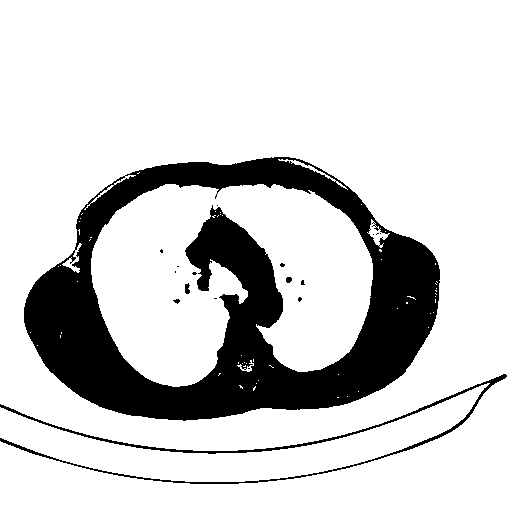
\includegraphics[width=2.9in]{imagens/TCpulmaoTHRESHOLDED.png}}
  \subfigure[Depois da remoção.]{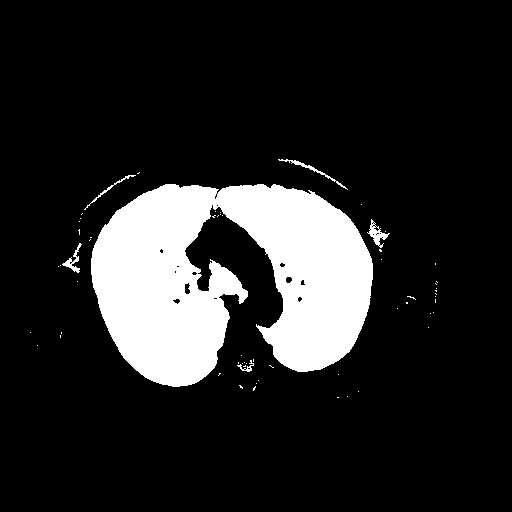
\includegraphics[width=2.9in]{imagens/TCpulmaoWOair.png}}
 \end{center}
 \caption{Imagem de TC antes e depois da remoção das partes que não pertencem ao corpo.}
 \label{fig:remocao}
\end{figure}

A eliminação das regiões que não fazem parte do pulmão é feita analisando-se todos os pixels que representam o pulmão (brancos) na imagem, de maneira que se a soma dos pixels vizinhos que representam o fundo (pretos) exceder em 2 ou mais a soma dos pixels vizinhos que representam o pulmão, então esse pixel se tornará parte do fundo. São considerados pixels vizinhos aqueles que se encontram no quadrado de 5x5 tendo como centro o pixel analisado.

Esse procedimento é realizado até 40 vezes, ou seja, ele será executado uma vez, se algum pixel for alterado, ele será executado novamente, até que nenhum pixel seja alterado ou que ele já tenha se repetido 40 vezes, podemos ver um exemplo na fig.~\ref{fig:clean}.

\begin{figure}[!ht]
 \begin{center}
  \subfigure[Antes da limpeza.]{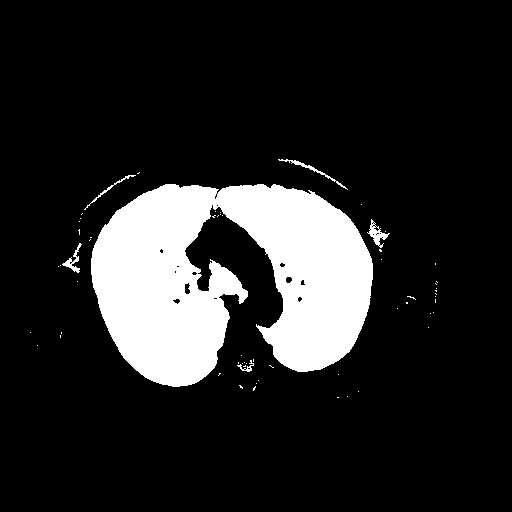
\includegraphics[width=2.9in]{imagens/TCpulmaoWOair.png}}
  \subfigure[Depois da limpeza.]{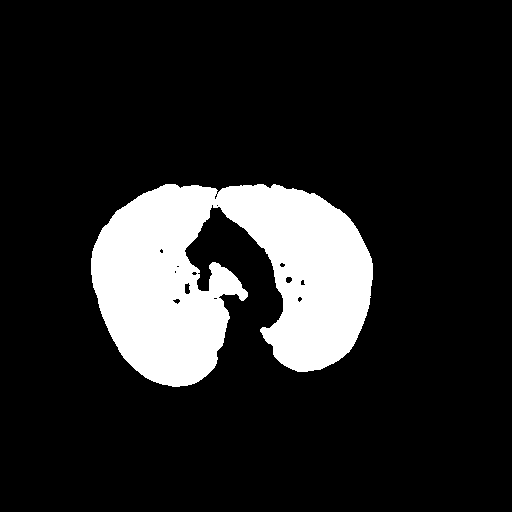
\includegraphics[width=2.9in]{imagens/TCpulmaoCleaning.png}}
 \end{center}
 \caption{Imagem de TC antes e depois da eliminação das regiões que não fazem parte do pulmão.}
 \label{fig:clean}
\end{figure}

Para remover os buracos dentro do pulmão e juntar pedaços separados de um mesmo pulmão, é realizado uma operação morfológica de fechamento utilizando como elemento estruturante um círculo de raio 6 pixels, como podemos ver na fig.~\ref{fig:fechamentoAplicado}. Essa operação pode causar com que pulmões muito próximos se juntem, tornando a próxima etapa ainda mais importante.

\begin{figure}[!ht]
 \begin{center}
  \subfigure[Antes do fechamento.]{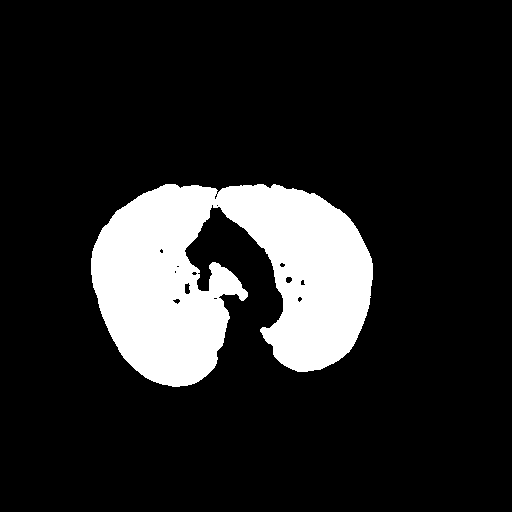
\includegraphics[width=2.9in]{imagens/TCpulmaoCleaning.png}}
  \subfigure[Depois do fechamento.]{
\includegraphics[width=2.9in]{imagens/TCpulmaoBinaryBall.png}}
 \end{center}
 \caption{Imagem de TC antes e depois da operação morfológica de fechamento utilizando um círculo de raio 6 pixels.}
 \label{fig:fechamentoAplicado}
\end{figure}

Para identificar os pulmões primeiro verifica-se quantas regiões conectadas existem, se existir apenas uma, realiza-se uma busca a partir do centro da imagem pela coluna que possuir menos pixels que representam o pulmão, sendo que a busca para quando a quantidade desses pixels começa a aumentar. Com essa estratégia paramos o algoritmo antes de encontrarmos estruturas pulmonares menores. Podemos ver um exemplo dessa etapa na fig.~\ref{fig:separacao}.

\begin{figure}[!ht]
 \begin{center}
  \subfigure[Pulmões juntos.]{
\includegraphics[width=1.9in]{imagens/TCpulmaoBinaryBall.png}\label{fig:separacao:a}}
  \subfigure[Pulmão esquerdo.]{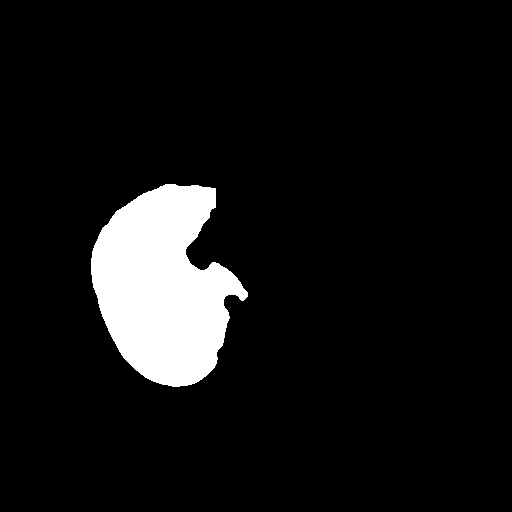
\includegraphics[width=1.9in]{imagens/TCpulmaoEsquerdo.png}\label{fig:separacao:b}}
  \subfigure[Pulmão direito.]{
\includegraphics[width=1.9in]{imagens/TCpulmaoDireito.png}\label{fig:separacao:c}}
 \end{center}
 \caption{Pulmões unidos em \ref{fig:separacao:a}, e depois devidamente separados e identificados em \ref{fig:separacao:b} e \ref{fig:separacao:c}.}
 \label{fig:separacao}
\end{figure}

\subsection{Recuperação de imagens baseada em conteúdo}

Primeiramente foi necessário escolher as características a serem utilizadas para o cálculo de similaridade, as quais foram energia, entropia, correlação, constraste e momento diferencial inverso.

Com isso é preciso que a RNA tenha 10 nodos de entrada, 5 para cada vetor de características. E como a saída da RNA é o valor de similaridade, ela possui apenas um nodo de saída. Para que tenhamos um valor entre 0 e 1 na saída, foi utilizada a seguinte função sigmóide:

\begin{equation}
	y = \frac{1}{1 + e^{-x}}
\end{equation}

A qual é derivada na equação~\ref{equa:sigmoide:derivada}, que tem custo computacional baixo, pois como utilizamos para aprendizado o algoritmo de retro-propagação, o valor de $y$ não precisa ser calculado novamente na atualização dos pesos.

\begin{equation}
	y \cdot (1 - y)
	\label{equa:sigmoide:derivada}
\end{equation}

A RNA foi dimensionada com 2 camadas intermediárias, sendo que na primeira camada temos 11 nodos e na segunda camada 13 nodos.

A taxa de aprendizado escolhida para o algoritmo de retro-propagação é 0,2. O valor de $o_j$, que é o valor de saída esperado, na equação~\ref{equa:back:output} é 1 se o usuário considerar as imagens comparadas similares, 0 se considerar diferentes e 0,5 se não for considerada igual nem diferente.

O treinamente é realizado com um conjunto de imagens de 20 pacientes. Que é repetido até 1000 vezes ou até que o erro médio do conjunto de imagens seja menor que 0,001. Alguns pares no conjunto de imagens de treinamento foram montados de modo a fazer com que a RNA seja associativa entre duas imagens, ou seja, se a similaridade de uma imagem $x$ com uma imagem $y$ for $z$, então a similaridade entre a imagem $y$ e a imagem $x$ também deve ser $z$. Também foram feitos pares no conjunto de imagens de treinamento com a mesma imagem, pois nesse caso o resultado deve ser, idealmente, 1.